\subsection{Introduction}

Marco: secondo me, vale subito la pena dire che questo caso ha una minor potenzialita' di scoperta ( a causa della luminosita' minore), ma in caso di segnale puo' meglio misurarne le caratteristiche (risoluzione e polarizzazione)
I due casi sono complementari! (missing e' come scoperta, e MesonEx come studio dello stato risonante)

\subsection{General features of the $\gamma^* p \rightarrow X \rightarrow J/\psi \, p$ reaction in MesonEx}

Before discussing in details the measurement $\gamma^* p \rightarrow X \rightarrow J/\psi \, p$ reaction in the MesonEx experiment, we want to briefly discuss some general features, that show the potentiality of this experiment searching for resonances decaying in the $J/\psi\, p$ final state. 

We consider the quasi-real photo-production reaction $e~p~\rightarrow~\gamma^*~p~e^{\prime}~\rightarrow~J/\psi~p~e^{\prime}$, with the final stat electron scattered at low angle and measured in the Forward Tagger detector. The final state proton and the $J/\psi$ decay products, instead, are measured in the CLAS12 detector.

In this analysis, we focused only in the $J/\psi$ decay to an electron-positron pair. We do not consider the $\mu^+ \mu^-$ decay channel, that as a comparable branching ratio, since the CLAS12 detector is not equipped with a muon identification system and, therefore, pion background would probably be too high to clearly identify the $J/\psi$ signal.


\paragraph{Invariant mass resolution: } the invariant mass $W$ of the $J/\psi\, p$ system can be measured in MesonEx as the missing mass of the final state electron, that depends only from the measured energy of the electron in Forward Tagger. Explicitly,
\begin{equation}
W^2=M_p^2+2E_0M_P-2E^{\prime}M_p \; \; ,
\end{equation}
with $E_0$, $E^{\prime}$ the primary beam energy and the final state electron energies. In particular, for $W=4449.8$ MeV (mass of the narrower $P_c$ state), $E^{\prime}=917.7$ MeV ($E^*_{\gamma}=10.08$ GeV).
Therefore, close to the mass region where resonances are expected, one has:
\begin{equation}
\sigma_W=\sigma_{E^{\prime}} \cdot \frac{M_p}{W} \simeq 0.21 \cdot \sigma_{E^{\prime}} \simeq \mbox{ 5.2 MeV}\; \; ,
\end{equation}  
being $\sigma_{E^{\prime}} \simeq$ 25 MeV the expected energy resolution for the final state electron measured in the Forward Tagger Detector \cite{Celentano:2014boa} for $E^\prime \simeq 1$ GeV. 
This value is significantly lower than the resonance width reported by LHCB for the narrower $P_c$ state, $\Gamma_a=39$ MeV, demonstrating that MesonEx is, in principle, capable of properly determining the resonance line-shape.
\paragraph{Number of measured events: } in the low $Q^{2}$ limit, the unpolarized differential reaction cross-section, with respect to the scattered electron angle $\Omega^{\prime}$ and energy $E^{\prime}$ in the laboratory frame, is \cite{Budnev:1974de}:
\begin{equation}
d\sigma(\Omega^{\prime},E^{\prime}) = \sigma_\gamma(\nu) \cdot d \Psi(\Omega^{\prime},E^{\prime}) \; \; ,
\end{equation}
with $\sigma_\gamma(\nu)$ the \textit{total} cross section for the real photo-production reaction $\gamma p \rightarrow J/\psi\, p$, being $\nu$ the virtual photon energy. The term $d \Gamma(\Omega^{\prime},E^{\prime})$ is the equivalent photon flux, given by:
\begin{equation}
d\Gamma(\Omega^{\prime},E^{\prime})=\frac{\alpha}{4\pi^{2}}\frac{E^{\prime}}{E_0}\frac{\nu}{Q^2}\left[\frac{(2E_0-\nu)^2}{\nu^2}+1  \right] d\Omega^{\prime} \,d E^{\prime}
\end{equation}
To obtain the angular-integrated photon flux, the Forward Tagger nominal acceptance has to be considered, i.e. $2.5^{\circ}<\theta^{\prime}<4.5^{\circ}$. This gives:
\begin{equation}
d\Gamma(E^{\prime})=\frac{\alpha}{4\pi}\frac{\nu}{E^2_0}\left[\frac{(2E_0-\nu)^2}{\nu^2}+1  \right] \log{ \left( \frac{1-\cos\theta_{max}}{1-\cos\theta_{min}}      \right)} d E^{\prime} \simeq 1.1 \cdot \frac{\alpha}{4\pi}\frac{\nu}{E^2_0}\left[\frac{(2E_0-\nu)^2}{\nu^2}+1  \right] d E^{\prime}
\end{equation}
To compare with the previous case (experiment E12-12-001, with the low-angle scattered electron identified in missing momentum analysis), we re-write the flux as a function of $W$:
\begin{equation}
d\Gamma(W) \simeq 1.1 \cdot \frac{\alpha}{4\pi}\frac{\nu}{E^2_0}\left[\frac{(2E_0-\nu)^2}{\nu^2}+1  \right]\frac{W}{M_p}dW
\end{equation}

At $W=4.4$ GeV, integrating over $\Delta_W=20$ MeV, this results in $\Gamma/e=1.23\cdot 10^{-5}$, an order of magnitude lower than the corresponding value in E12-12-001: 
this is a direct consequence of the lower cut-off on the $\theta^{\prime}$ angle imposed by the FT acceptance.

A reasonable estimate for the number of expected events for a resonant signal can be obtained by assuming a constant photo-production cross-section $\sigma^{\gamma}_0$, equal to the value at the resonance mass, 
and integrating in the electron energy range corresponding to the mass interval $(M-\Gamma/2,M+\Gamma/2)$, i.e. 825.1 MeV $<$ $E^{\prime}$ $<$ 1010.0 MeV for the narrower $P_c$ state ($M=4450$ MeV and $\Gamma=39$ MeV).

The foreseen rate of produced events, considering the nominal CLAS12 luminosity, $\mathcal{L}=10^{35} cm^{-2} s^{-1}$, is therefore:
 \begin{equation}
R_{gen} = \mathcal{L} \cdot \Gamma \cdot \sigma^{\gamma}_0 \simeq 2 \cdot 10^5 \cdot \sigma^{\gamma}_0 \mbox{ events / day / }\mu{\mbox barn}
\end{equation}

To get the actual number of measured events, this has to be multiplied by the branching fraction for the decay $J/\psi\rightarrow e^{+} e^{-}$ ($\simeq 5.9\%$). 
Finally, the CLAS12 acceptance $\varepsilon$ has to be considered: as discussed below, the value obtained from MonteCarlo simulations is $\varepsilon \simeq 0.13$, if all the final state particles (proton and electron-positron pair) are detected, and slightly higher if only the two leptons are measured, the proton being reconstructed via missing mass technique. This gives:
\begin{eqnarray}
R_{meas} &=& R_{gen} \cdot BR_{J/\psi\rightarrow e^{+}e^{-}} \cdot \varepsilon \simeq 1.5 \cdot 10^{3}  \cdot \sigma^{\gamma}_0 \mbox{ events / day / }\mu{\mbox barn}\\
 N_{meas} &\simeq& 1.2\cdot10^5 \cdot \sigma^{\gamma}_0 / \mu\mbox{barn} \; \; \; ,
\end{eqnarray}
considering the nominal MesonEx run time of 80 days. 

From this, a preliminary estimate of the experiment sensitivity can be derived, by requiring to have $\simeq$ 1000 events in total, i.e. $\simeq 50$ events / $W-bin$, assuming $\Delta_W=5$ MeV (the experimental resolution), and $\simeq 20$ bins 
(to properly measure the narrower $P_c$ state). The corresponding experimental sensitivity to a resonant signal is $\simeq$ 10 nbarn.


\subsection{Kinematics}
 
To simulate the measurement of the reaction $\gamma^* p \rightarrow J/\psi \, p$ with the CLAS12+Forward Tagger detector, we generated a large set of events trough a proper model, that includes two contributions:
\begin{itemize}
\item{A non-resonant production mechanism, parametrized via the $t-$channel exchange of a Pomeron trajectory. All the corresponding parameters, including the overall normalization, were tuned to reproduce the experimental data measured at higher energy  ($E_{\gamma} > 13$ GeV) \cite{Camerini:1975cy}.
We note, however, that the extrapolation of the total cross-section from the higher energy range where experimental data exist to the MesonEx range, close to the threshold, is very sensitive to the choice of the parameters. 
Specifically, with the actual values we used, we got $\sigma_{NR}(E_{\gamma}=10 \mbox{ GeV} ) = 0.2 $ nbarn \footnote
{
We observe that this value is compatible with the range predicted in \cite{bchl}, where a QCD-inspired calculation was performed.}.
} 
\item{A resonant production mechanism  , $\gamma^* p \rightarrow X \rightarrow J/\psi \, p$. 
In this note, we focused only on the narrower state reported by the LHCB experiment, $P_c(4450)$, leaving a proper study of the measurement feasibility as a function of the $X$ mass and width for the future. 
Furthermore, in the development of the production model, we only considered the $J^P$ assignment $(3/2)^-$, although we verified that this has a very limited impact on the foreseen experimental acceptance. 

This contribution is characterized by a single free parameter, the branching ratio BR of the decay $X \rightarrow J/\psi \, p$. 
The total cross section at the resonance peak reads: $\sigma_{R}(E_{\gamma}=10 \mbox{ GeV} ) = (BR)^{2}\cdot 1.3 \, \mu$barn. 
In this note, we considered the case BR $\simeq$ 0.1, so that $\sigma_{R}~\simeq~ 13$ nbarn at the resonance peak.}
\end{itemize}

The distribution of the  $J/\psi \, p$ invariant mass ($W$) is reported in Fig.~\ref{fig:1}, together with the correlation between $W$ and the momentum transferred on the proton, $-t$. 
In the production model that we developed, the $X\rightarrow J/\psi \, p$ decay is almost isotropic in the CM frame, due to the barrier-factor effects in the proximity of the $J/\psi \, p$ threshold.
 The non-resonant contribution, instead, is characterized by a diffractive-like $t$ dependence, $d\sigma / d t~\propto~\exp(- b \cdot |t|)$, with $b\simeq 2.8$ \cite{Camerini:1975cy}.

The momentum-against-angle distribution for proton and leptons, in the laboratory frame, is plotted in Fig.~\ref{fig:2}. 
The proton is always emitted at low angle, $\theta_P < 25^{\circ}$, due to the lower mass with respect to the $J/\psi$ meson. 
The $e^{+}$ and the $e^{-}$, instead, are typically emitted at larger angle, with a significant fraction of events with one or both out of the CLAS12-FD acceptance.
\begin{figure}[tpb]
\subfigure{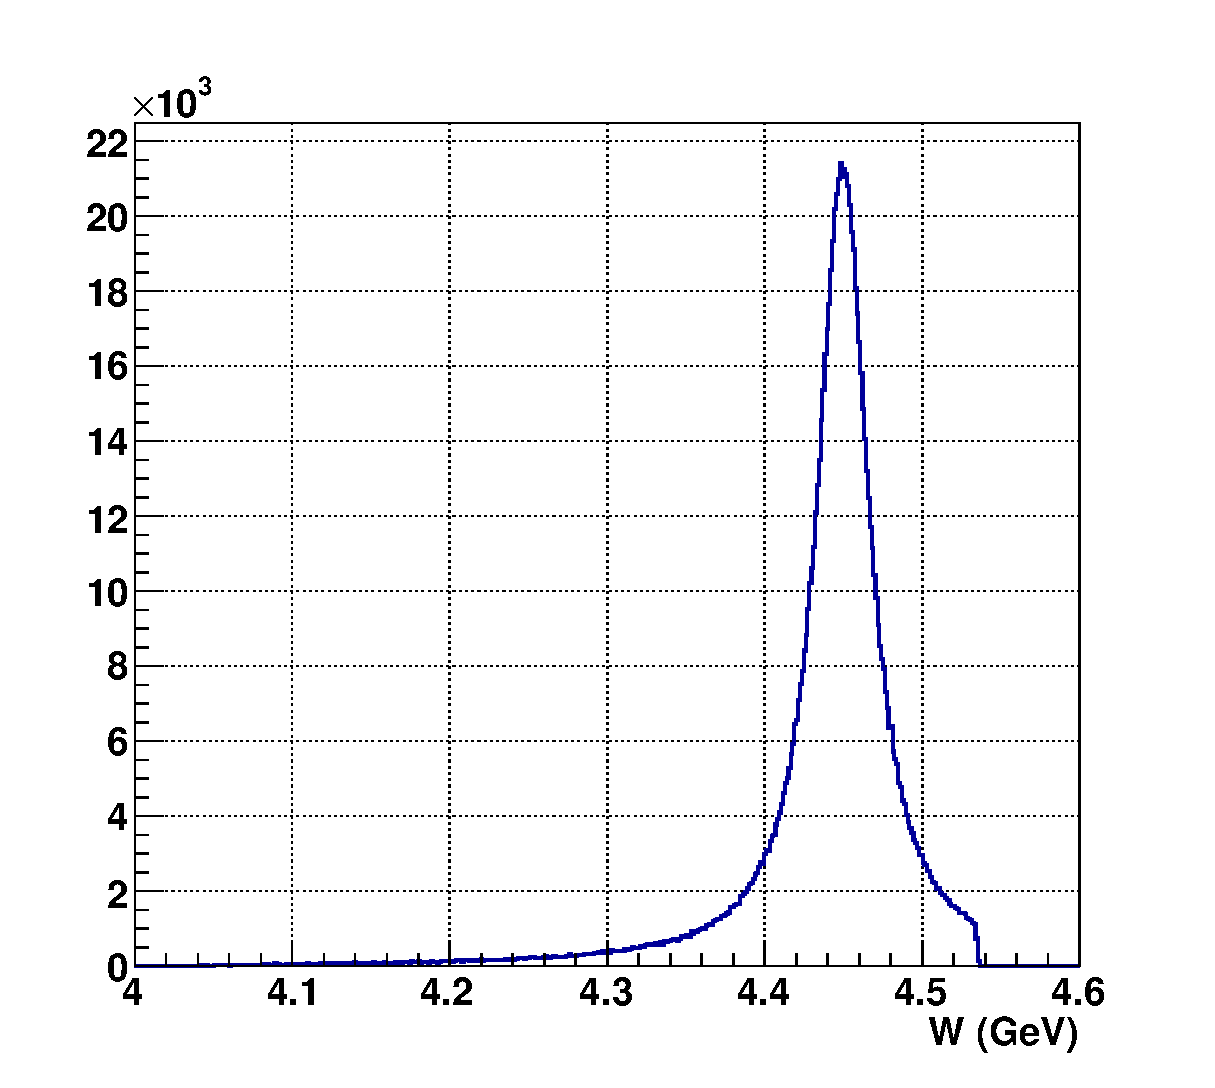
\includegraphics[width=0.45\textwidth]{WGEN.eps}}
\subfigure{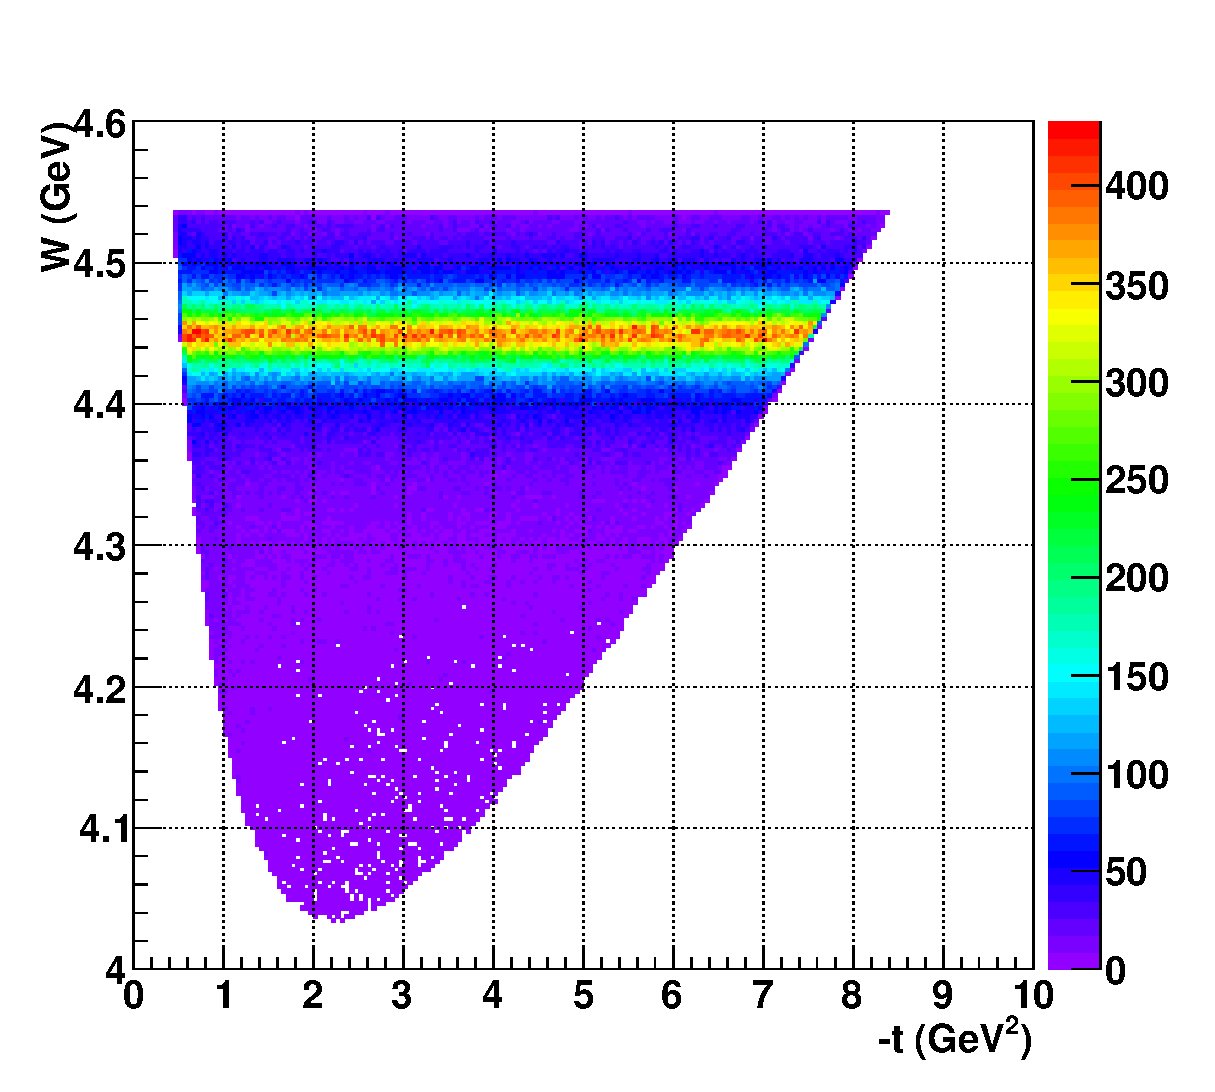
\includegraphics[width=0.45\textwidth]{WvstGEN.eps}}
\caption{\footnotesize \label{fig:1} Left: $J/\psi \, p$ invariant mass distribution. Right: $J/\psi \, p$ invariant mass vs momentum transfer on the proton distribution.}
\end{figure}

\begin{figure}[tpb]
\subfigure{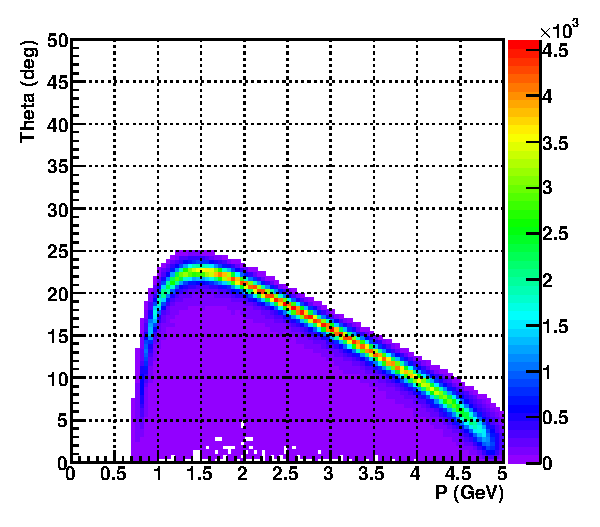
\includegraphics[width=0.45\textwidth]{protonGEN.eps}}
\subfigure{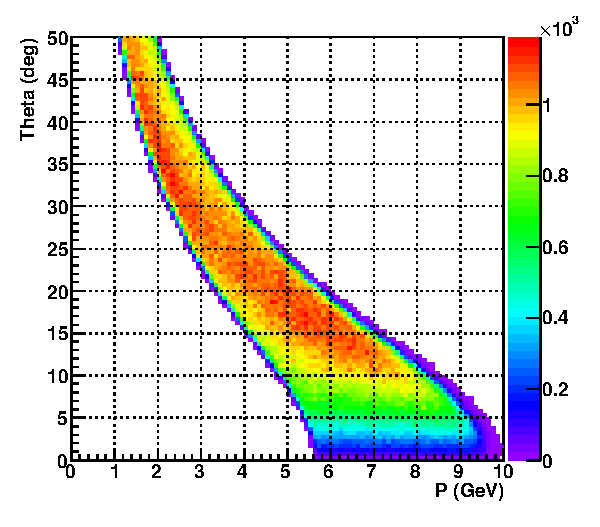
\includegraphics[width=0.45\textwidth]{leptonGEN.eps}}
\caption{\footnotesize \label{fig:2} Momentum-against-angle distribution for the final state proton (left) and for the leptons (right), in the laboratory frame.}
\end{figure}




\subsection{Detector response}

The reaction that we consider foresees 4 particles in the final state: a low-angle scattered electron, measured with the Forward Tagger facility, and a proton and an electron-positron pair from $J/\psi$ decay, measured with the CLAS12 detector. Since the CLAS12-Central Detector (CD) is not suited for electron detection and identification, we consider only the detection of final state leptons in the CLAS12-Forward Detector (FD). Two possible measurement strategies are possible:
\begin{itemize}
\item{Measure \textit{all} the final state particles, reconstructing the $J/\psi$ via the invariant mass of the electron-positron pair.}
\item{Measure \textit{only} the scattered electron in the Forward Tagger and the electron-positron pair in CLAS12-FD, reconstructing the $J/\psi$ via the invariant mass of the $e^{+} e^{-}$ system and the proton via the missing mass on it.}
\end{itemize} 
While the first solution would permit a better background discrimination, given the larger control on kinematics variable that the full measure of the final state permits, the second results in a slightly larger experimental acceptance. A proper discussion on the best measurement strategy would require a full simulation of the backgrounds associated with the measurement, not performed in this note: for this reason, in the following we will discuss both strategies. 

The CLAS12 and Forward Tagger response was simulated using the Fast MonteCarlo (FASTMC) software, that effectively accounts for the detector geometrical acceptance and resolution. Each final state particle, i.e. the recoil
proton, the scattered electron, and the two leptons, is projected individually on the detector. If it is within the nominal detector acceptance region, the four-momentum is smeared according to the expected resolution, otherwise it is discarded. We made the following conservative assumptions:
\begin{itemize}
\item{The CLAS12-CD acceptance for leptons is zero. As discussed, this reflects the fact that this detector is not designed for $e^- / e^+$ detection and identification.}
\item{We considered only events with both the electron and the positron from $J/\psi$ decay detected in the CLAS12-CD, i.e. we neglected the possibility that they are measured with the Forward Tagger.}
\end{itemize}

The resolution on the reconstructed $J/\psi$ mass, from the $e^{+} e^{-}$ measured four vectors, is reported in Fig.~\ref{fig:3}. At the maximum value of the CLAS12 toroidal field, with positive (negative) particles being outbended (inbeded), a resolution of $\simeq 15$ MeV is obtained, as shown in the left panel. The right panel, instead, reports the resolution on the $e^- - e^+$ missing mass, relevant for the second measurement strategy outlined before.

\begin{figure}[tpb]
\subfigure{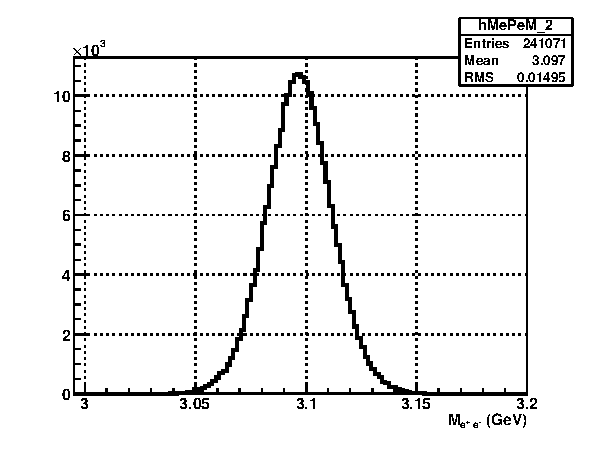
\includegraphics[width=0.45\textwidth]{resJPSInominal.eps}}
\subfigure{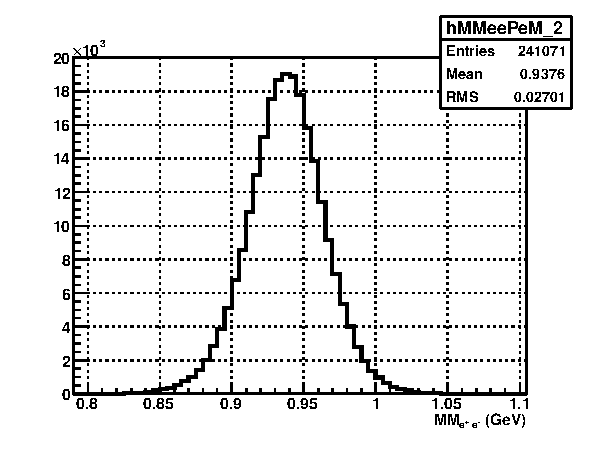
\includegraphics[width=0.45\textwidth]{resPnominal.eps}}
\caption{\footnotesize \label{fig:3} Left: reconstructed $J/\psi$ mass. Right: missing mass on the $e^+\,e^-$ pair. Both plots refer to the maximum value of the CLAS12 toroidal field, configured to have positive particles outbending.}
\end{figure}

We also investigated the effect of a magnetic field variation on the above quantities. As expected, we observed that there is almost no dependence on the orientation of the CLAS12 toroidal field, given the charge symmetry of the $e^+ e^-$ system. Results are reported in Fig.~\ref{fig:4}.

\begin{figure}[tpb]
\subfigure{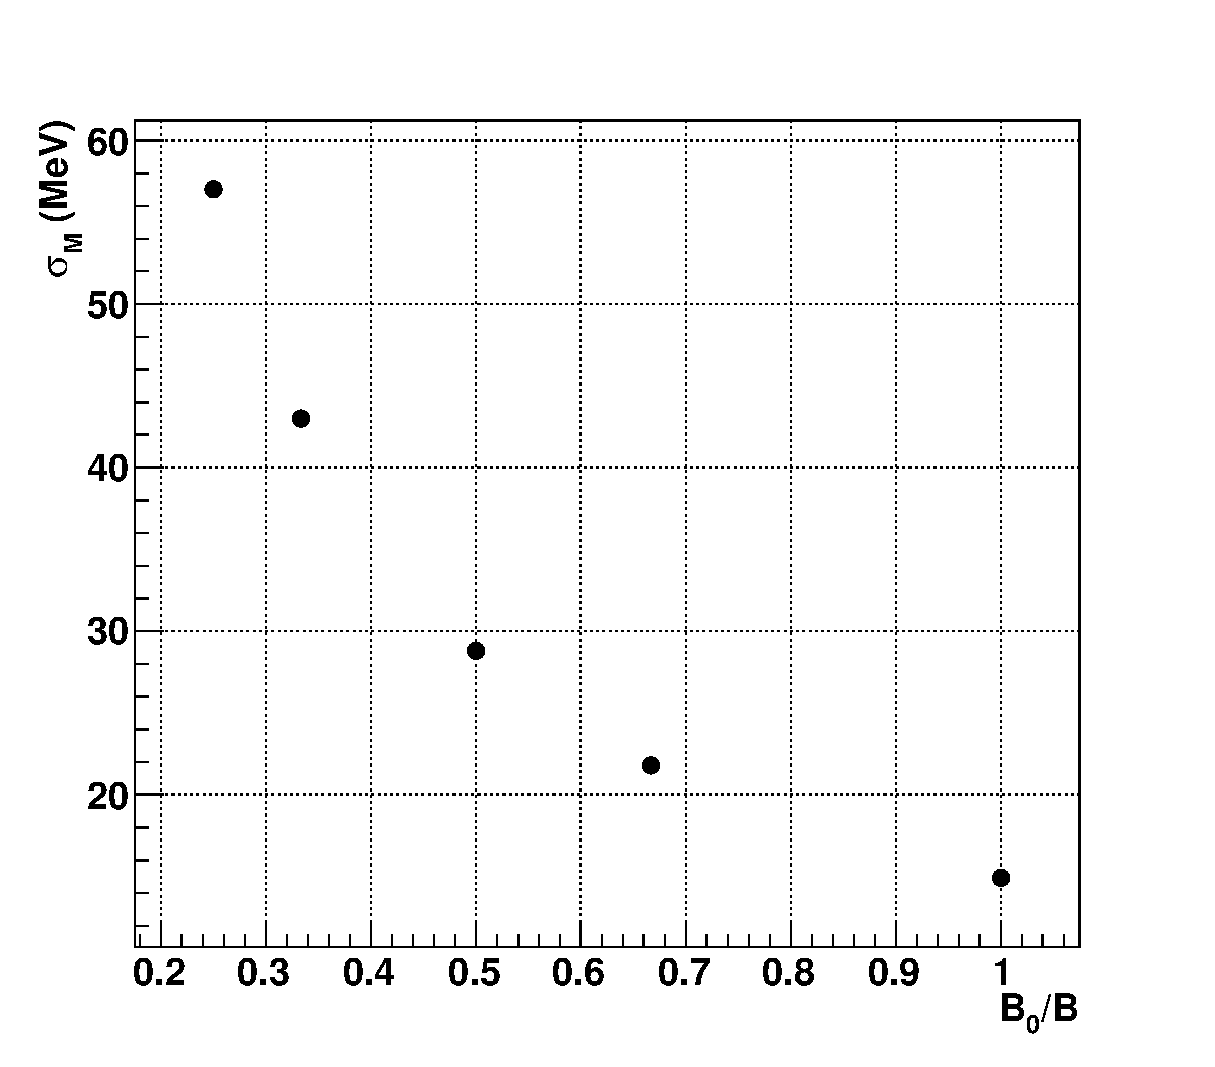
\includegraphics[width=0.45\textwidth]{resJPSIfield.eps}}
\subfigure{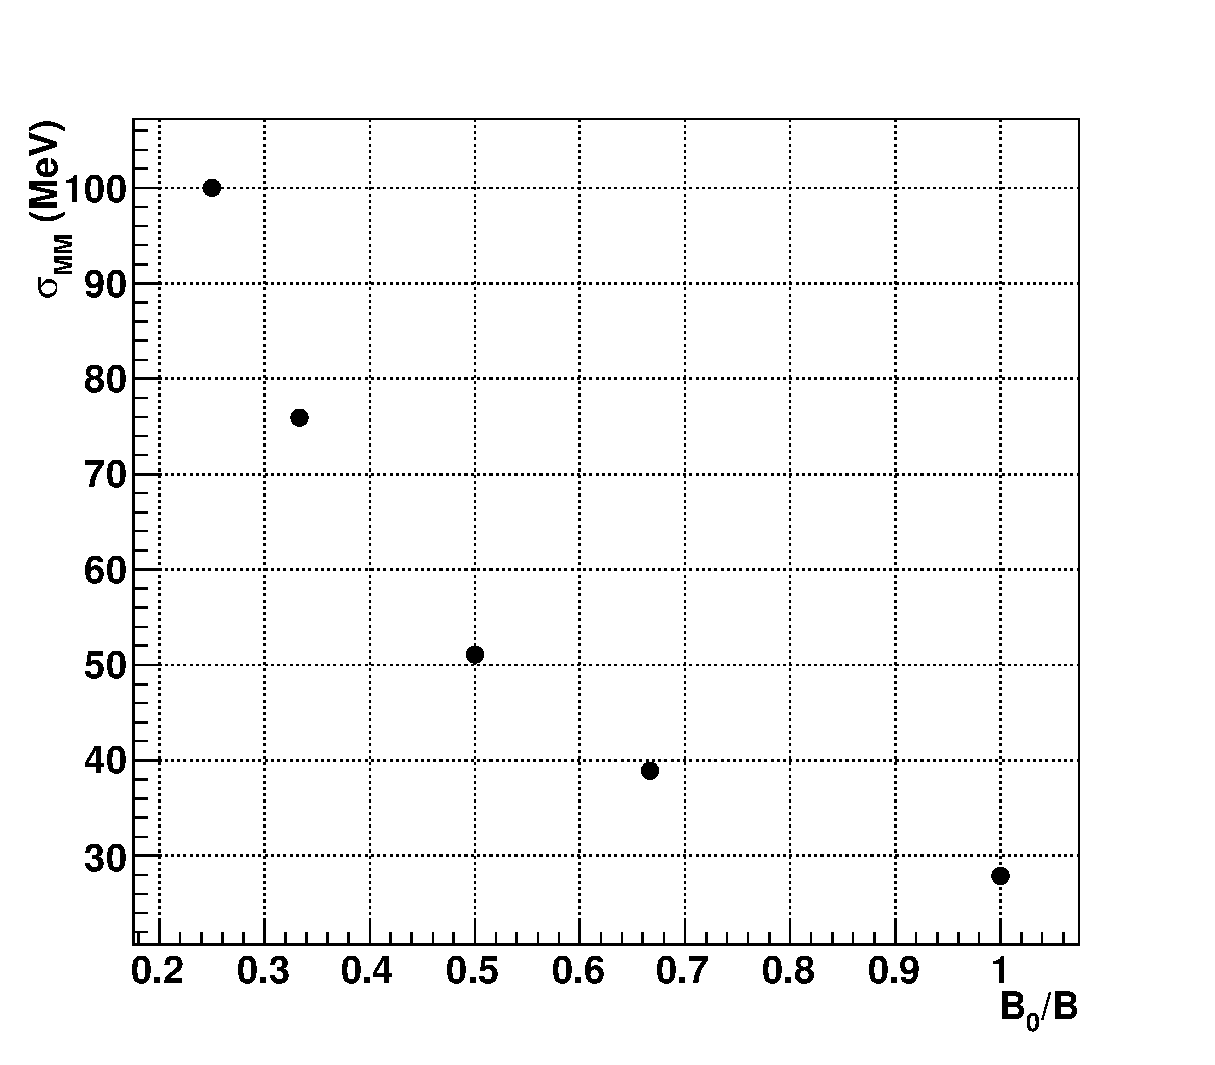
\includegraphics[width=0.45\textwidth]{resPfield.eps}}
\caption{\footnotesize \label{fig:4} Left: reconstructed $J/\psi$ mass resolution as a function of the CLAS12 toroidal field intensity (normalized to the maximum possible value). Right: resolution on the missing mass on the $e^+\,e^-$ pair as a function of the CLAS12 toroidal field intensity.}
\end{figure}

The CLAS12 acceptance, as a function of the $J/\psi\, p$ invariant mass $W$, is reported in Fig.~\ref{fig:5}, for both measurement strategies outlined below. For both cases, the acceptance shows a smooth increase with $W$, with an average value of $\simeq 13\%$ for the detection of all final state particles ($\simeq 16\%$ for the detection of the $e^{+} e^{-}$ pair only). We observe that the ``deep'' at $W=4.4$ GeV, at the resonance mass, is due to the fact that resonance production mechanism is characterized by a very different kinematics than the background, in particular for the $t$ dependence, and, therefore, the corresponding CLAS12 response is different. 

We also investigated the effect of a change in the CLAS12 toroidal field, finding a very modest dependence on in. 
The larger effect comes from inverting the polarity of the field, i.e. having the proton being inbended by the field. In this case, the acceptance for the measure of all the final state particles drops to $\simeq 9\%$, while there is no change for the measure of the $e^+ e^-$ pair only.

\begin{figure}[tpb]
\center
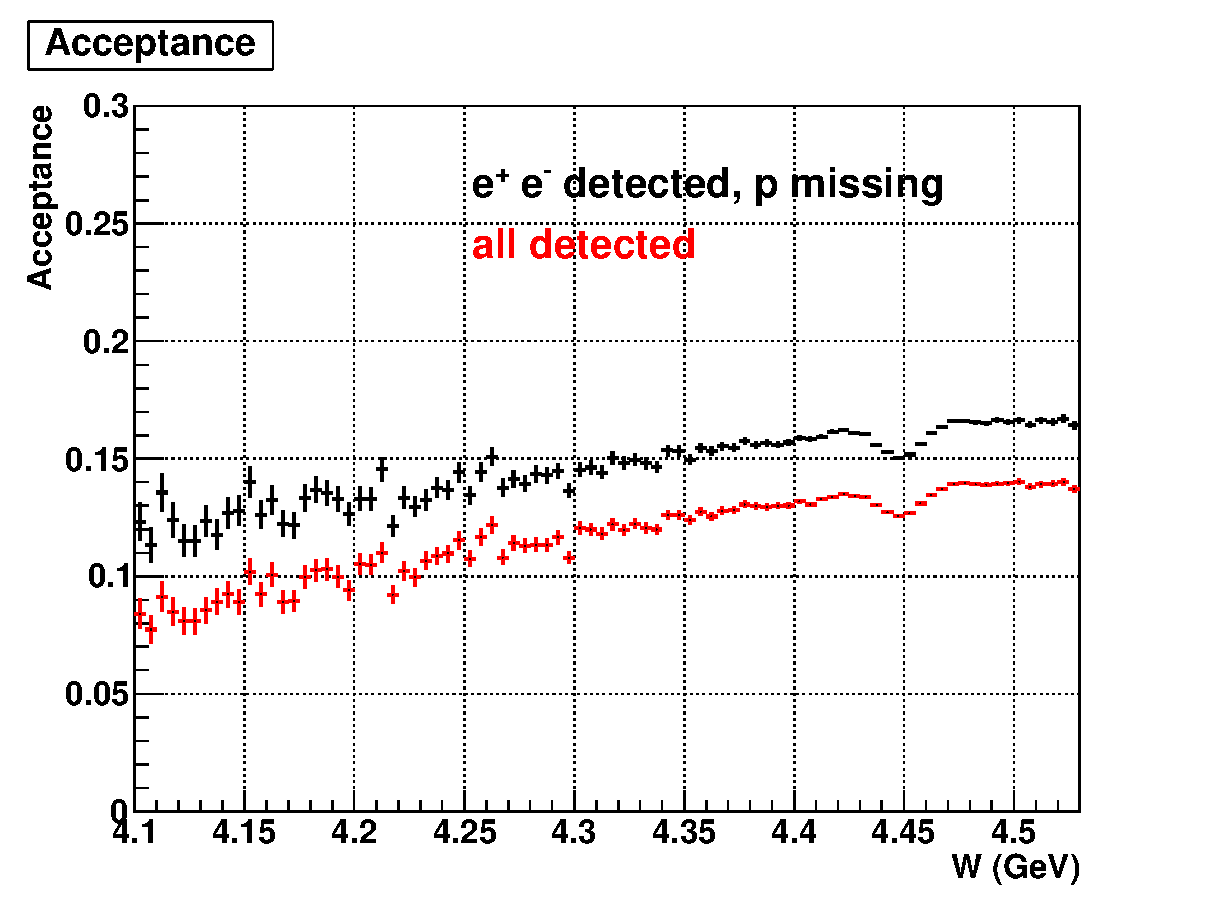
\includegraphics[width=0.7\textwidth]{acceptanceNominal.eps}
\caption{\footnotesize \label{fig:5} Detector acceptance as a function of the  $J/\psi\, p$ invariant mass, for both measurement strategies outlined before. Both plots refer to the maximum value of the CLAS12 toroidal field, configured to have positive particles outbending. }
\end{figure}

Finally, the resolution on the $J/\psi\, p$ invariant mass $W$, \textit{measured as the missing mass on the low-angle scattered electron}, is shown in Fig.~\ref{fig:6}. As pointed before, this quantity depends only on the measurement of the final state electron with the Forward Tagger calorimeter, and it is almost insensitive to the CLAS12 configuration. For $W=4.4$ GeV, $\sigma_W=5.5$ MeV, in agreement with the previous estimate.

\begin{figure}[tpb]
\center
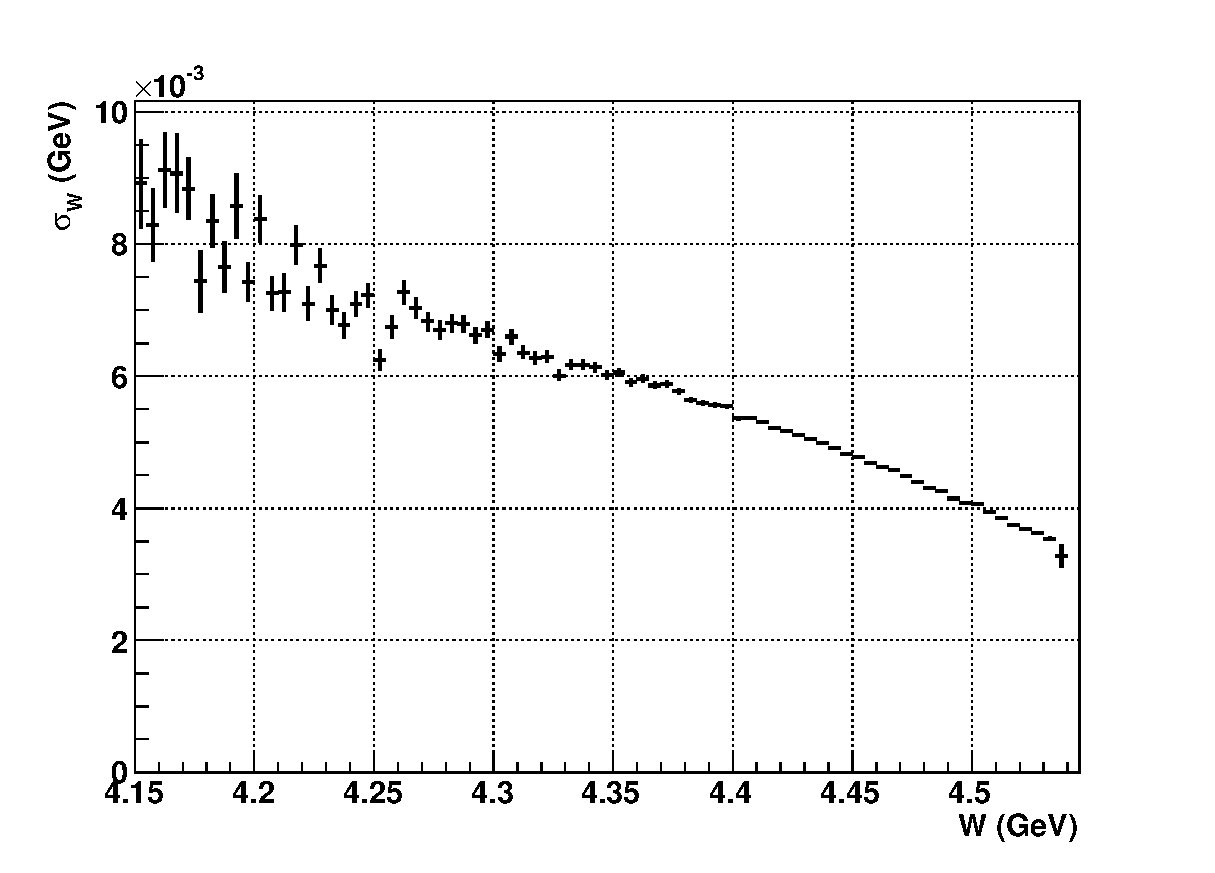
\includegraphics[width=0.7\textwidth]{resolutionW.eps}
\caption{\footnotesize \label{fig:6} Resolution on the  $J/\psi\, p$ invariant mass.}
\end{figure}








